\section{Introduction}

To recognize context-free languages we need an automaton with an auxiliary structured as an unbounded stack of symbols. 
The following operations apply to a stack:
\begin{itemize}
    \item Push: places the symbol(s) onto the stack top. 
    \item Pop: removes symbol from the stack top, if the stack is not empty; otherwise reads $Z_0$. 
    \item Stack emptiness test: true if the stack is empty, false otherwise. 
\end{itemize}
The symbol $Z_0$ is the stack bottom and can be read but not removed. 
The symbol $\dashv$ is the terminator character of the input string.

The configuration is specified by: current state, current character, and stack contents. 
With a move the pushdown automaton: 
\begin{itemize}
    \item Reads the current character and shifts the input head, or performs a spontaneous move without shifting the input head. 
    \item Reads the stack top symbol and removes it from the top if the stack is not empty, or reads the stack symbol $Z_0$ if the stack is empty. 
    \item Depending on the current character, state and stack top symbol, it goes into the next state and places none, one or more symbols onto the stack top. 
\end{itemize}
\begin{definition}
    A pushdown automaton $M$ is defined by:
    \begin{itemize}
        \item $Q$ a finite set of states of the control unit.
        \item $\Sigma$ a finite input alphabet.
        \item $\Gamma$ a finite stack alphabet.
        \item $\delta$ a transition function.
        \item $q_0 \in Q$ the initial state.
        \item $Z_0 \in \Gamma$ the initial stack symbol.
        \item $F \subseteq Q$ a set of final states.
    \end{itemize}
\end{definition}
The transition function $\delta$ has:
\begin{itemize}
    \item Domain: $Q \times \left(\Sigma \cup \{\varepsilon\}\right) \times \Gamma$. 
    \item Image: the set of the subsets of $Q \times \Gamma^{*}$. 
\end{itemize}
The possible moves are: 
\begin{itemize}
    \item Reading move: in the state $q$ with symbol $Z_0$ on the stack top, the automaton reads char $a$ and enters one of the states $p_i$ with $1 \leq i \leq n$, after orderly executing the operations pop and push ($\gamma_i$): 
        \[\delta(q,a,Z)=\{(p_1,\gamma_1), (p_2,\gamma_2),\dots,(p_n,\gamma_n)\}\]
    \item Spontaneous move: in the state $q$ with symbol $Z_0$ on the stack top, the automaton does not read any input character and enters one of the states $p_i$ with $1 \leq i \leq n$, after orderly executing the operations pop and push ($\gamma_i$): 
        \[\delta(q,\varepsilon,Z)=\{(p1,\gamma_1), (p2,\gamma_2),\dots,(p_n,\gamma_n)\}\]
\end{itemize}
\begin{table}[H]
    \centering
    \begin{tabular}{ccc}
    \hline
    \textbf{Current configuration} & \textbf{Next configuration} & \textbf{Applied move} \\ \hline
    $(q,az,\eta Z)$                & $(p,z,\eta\gamma)$          & Reading               \\
    $(q,az,\eta Z)$                & $(p,az,\eta\gamma)$         & Spontaneous           \\ \hline
    \end{tabular}
\end{table}

There is non-determinism: for a triple (state, input, stack top) there are two or more possible moves that consume none or one input character. 

\begin{definition}
    The \emph{instantaneous configuration} of a machine $M$ is a 3-tuple: 
    \[(q,y,\eta)\in Q \times \Sigma^{*} \times \Gamma^{+}\]
    which specifies:
    \begin{itemize}
        \item $q$: the current state of the control unit. 
        \item $y$: the part of the input string $x$ that still has to be scanned.
        \item $\eta$: the current contents of the pushdown stack.
    \end{itemize}

    The \emph{initial} configuration of machine $M$ is: 
    \[(q_0,x,Z_0)\]

    The \emph{final} configuration of machine $M$ is: 
    \[(q,\varepsilon,\lambda)\]
\end{definition}

Applying a move, a transition from a configuration to another occurs, to be denoted as: 
\[(q,y,\eta)\rightarrow(p,z,\lambda)\]
Note that a chain of one or more transitions is denoted by $\overset{+}{\rightarrow}$. 

An input string $x$ is accepted by final state if there is the following computation:
\[(q_0,x,Z_0)\overset{*}{\mapsto}(q,\varepsilon,\lambda)\]
where $q \in F$ and $\lambda\in\Gamma^{*}$, whereas there is not any specific condition for $\lambda$; sometimes $\lambda$ happens to be the empty string, but this is not necessary. 

\subsection*{State-transition graph}
The transition function of a finite automaton can be graphically represented.
The numerator indicates the characters read in the input tape and in the memory. 
The denominator indicates the replacement for the element in the stack memory. 
\begin{example}
    The language $L=\{uu^R|u \in \{a,b\}^{*}\}$ of the palindromes of even length is accepted with final state by the pushdown recognizer. 
    \begin{figure}[H]
        \centering
        \includegraphics[width=0.5\linewidth]{images/pda.png}
    \end{figure}
\end{example}

\subsection*{From grammar to pushdown automata}
Grammar rules can be viewed as the instructions of a non-deterministic pushdown automaton. 
Intuitively such an automaton works in a goal-oriented way and uses the stack as a notebook of the sequence of actions to undertake in the next future. 

The stack symbols can be both terminals and non-terminals of the grammar. 
If the stack contains the symbol sequence $A_1 \dots A_k$, then the automaton executes first the action associated with $A_k$, which should recognize if in the input string from the position of the current character $a_i$ there is a string w that can be derived from $A_k$; if it is so, then the action shifts the input head of $\left\lvert w\right\rvert $ positions. 

An action can be recursively divided into a series of sub-actions, if to recognize the non-terminal symbol $A_k$ it is necessary to recognize other non-terminals. 

The initial action is the grammar axiom: the pushdown recognizer must check if the source string can be derived from the axiom. 
Initially the stack contains only the symbol $Z_0$ and the axiom $S$, and the input head is positioned on the initial character of the input string. At every step the automaton chooses (non-deterministically) one applicable grammar rule and executes the corresponding move. 
The input string is recognized accepted when, and only when, it is completely scanned and the stack is empty. 
Given a grammar $G=(V,\Sigma,P,S)$ with $A,B \in V$, $b \in \Sigma$ and $A_i \in V \cup \Sigma$, the correspondence between a grammar and a pushdown automaton are summarized as follows: 

\begin{table}[H]
    \centering
    \begin{tabular}{|cc|}
    \hline
    \textbf{Grammar rule}                                      & \textbf{Automaton move}                                                                                    \\ \hline
    $A \rightarrow B A_1\dots A_n \textnormal{ with }n \geq 0$ & \makecell{If $\textnormal{top}=A$ then pop \\ Push $(A_n \dots A_1B)$}                                     \\ \hline
    $A \rightarrow b A_1\dots A_n \textnormal{ with }n \geq 0$ & \makecell{If $cc=b$ and $\textnormal{top}=A$ then pop \\ Push $(A_n \dots A_1)$ \\ Shift reading head}     \\ \hline
    $A \rightarrow \varepsilon$                                & If $\textnormal{top}=A$ then pop                                                                           \\ \hline
    For every character $b \in \Sigma$                         & \makecell{If $cc=b$ and $\textnormal{top}=b$ then pop \\ Shift reading head}                               \\ \hline
    ---                                                        & \makecell{If $cc=\dashv$ and the stack is empty then accept \\ Halt}                                       \\ \hline
    \end{tabular}
\end{table}
This construction may lead to a nondeterministic automaton. 
\begin{example}
    Consider the language $L=\{a^nb^m|n \geq m \geq 1\}$. 
    The nondeterministic grammar that generates the string of this language is as follows: 
    \[
    \begin{cases}
        S \rightarrow aS \\
        S \rightarrow A \\
        A \rightarrow aAb \\
        A \rightarrow ab
    \end{cases}
    \]
    Using the rules of the previous table we can construct the pushdown automaton in the following way: 
    \begin{table}[H]
        \centering
        \begin{tabular}{|ccc|}
        \hline
        $\#$ & \textbf{Grammar rule}    & \textbf{Automaton move}                                                                                   \\ \hline
        1    & $ S \rightarrow aS$      & \makecell{If $cc=a$ and $\textnormal{top}=S$ then pop \\ Push $S$ \\ Shift reading head}                  \\ 
        2    & $S \rightarrow A$        & \makecell{If $\textnormal{top}=S$ then pop \\ Push$(A)$   }                                               \\ 
        3    & $A \rightarrow aAb$      & \makecell{If $cc=a$ and $\textnormal{top}=A$ then pop \\ Push $bA$ \\ Shift reading head}                 \\ 
        4    & $A \rightarrow ab$       & \makecell{If $cc=a$ and $\textnormal{top}=A$ then pop \\ Push $b$ \\ Shift reading head}                  \\ 
        5    & ---                      & \makecell{If $cc=b$ and $\textnormal{top}=b$ then pop \\ Shift reading head}                              \\ 
        6    & ---                      & \makecell{If $cc=\dashv$ and the stack is empty then accept \\ Halt}                                      \\ \hline
        \end{tabular}
    \end{table}
\end{example}
The automaton recognizes a string if, and only if, the string is generated by the grammar: for every successful automaton computation there exists a grammar derivation and vice versa; thus the automaton simulates the leftmost derivations of the grammar.
However, the automaton cannot guess the correct derivation; it has to examine all the possibilities. 
A string is accepted by two or more different computations if and only if the grammar is ambiguous.

The construction from grammar to automaton can be inverted and used to obtain the grammar by starting from the pushdown automaton, if this is one-state.
\begin{property}
    The family of free languages generated by free grammars coincides with the family of the languages recognized by one-state pushdown automata.
\end{property}
Unfortunately in general the resulting pushdown automaton is non-deterministic, as it explores all the moves applicable at any point and has an exponential time complexity with respect to the length of the source string.

\subsection*{Varieties of pushdown automata}
The acceptance modes can be: 
\begin{enumerate}
    \item By final state: accepts when enters a final state independently of the stack contents. 
    \item By empty stack: accepts when the stack gets empty independently of the current state. 
    \item Combined: by final state and empty stack.
\end{enumerate}
\begin{property}
    For the family of (non-deterministic) pushdown automata with states, the three acceptance modes listed above are equivalent. 
\end{property}
A generic pushdown automaton may execute an unlimited number of moves without reading any input character. 
This happens if and only if it enters a loop made only of spontaneous moves. 
Such a behavior prevents it of completely reading the input string, or causes it to execute an unlimited number of moves before deciding whether to accept or reject the string.
Both behaviors are undesirable in the practice. 
It is always possible to build an equivalent automaton with no spontaneous loops. 

A pushdown automaton operates in on-line mode if it decides whether to accept or reject the string as soon as it reads the last character of the input string, and then it does not execute any other move. 
Clearly from a practical perspective the on-line mode is a desirable behavior.
It is always possible to build an equivalent automaton that works in on-line mode. 

\subsection*{Context-free languages and pushdown automata}
The language accepted by a generic pushdown automaton is free. 
Every free language can be recognized by a non-deterministic one-state pushdown automaton. 
\begin{property}
    The family of context-free languages coincides with that of the languages recognized by unrestricted pushdown automata. 
\end{property}
\begin{property}
    The family CF of context-free languages coincides with that of the languages recognized by the one-state non-deterministic pushdown automata.
\end{property}

\subsection*{Intersection of regular and context-free languages}
It is easy to justify that the intersection of a free and a regular language is free as well. 
Given a grammar $G$ and a finite state automaton $A$, the pushdown automaton $M$ that recognizes the intersection $L(G) \cap L(A)$ can be obtained as follows: 
\begin{enumerate}
    \item Construct the one-state pushdown automaton $N$ that recognizes $L (G)$ by empty stack. 
    \item Construct the pushdown automaton $M$ (with states), the state-transition graph of which is. 
        The Cartesian product of those of $N$ and $A$, by the Cartesian product construction so that the actions of $M$ on the stack are the same as those of $N$. 
\end{enumerate}
The obtained pushdown automaton $M$: 
\begin{enumerate}
    \item As its states, has pairs of states of the component machines $N$ and $A$. 
    \item Accepts by final state and empty stack (combined acceptance mode). 
    \item The states that contain a final state of $A$ are themselves final. 
    \item Is deterministic, if both component machines $N$ and $A$ are so. 
    \item Accepts by final state all and only the strings that belong to the intersection language.
\end{enumerate}
\begin{example}
    Consider the Dyck language $L=\{a^na^{'n}| n \geq 1\}$. 
    It is possible to construct a finite state automaton that recognizes the language by final state, that is: 
    \begin{figure}[H]
        \centering
        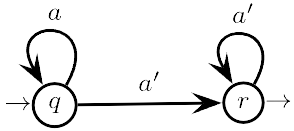
\includegraphics[width=0.25\linewidth]{images/pdaint.png}
    \end{figure}
    And also a pushdown automaton that recognizes the language by empty stack, that is: 
    \begin{figure}[H]
        \centering
        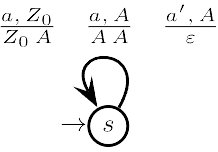
\includegraphics[width=0.25\linewidth]{images/pdaint1.png}
    \end{figure}
    By applying the intersection we obtain a product pushdown automaton that recognizes by empty stack in the final state $(r,s)$, that is: 
    \begin{figure}[H]
        \centering
        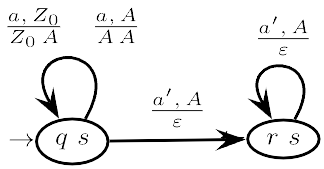
\includegraphics[width=0.3\linewidth]{images/pdaint2.png}
    \end{figure}
\end{example}